\documentclass[journal,twoside,web]{ieeecolor}


\usepackage{generic}
\usepackage{cite}
\usepackage{amsmath,amssymb,amsfonts}
\usepackage{algorithmic}
\usepackage{graphicx}
\usepackage{textcomp}
\usepackage{tabularray}
\usepackage{color}
\usepackage{booktabs}
\usepackage{graphicx}
\usepackage{array}
\usepackage{multirow}
\renewcommand{\arraystretch}{1}
\usepackage[T1]{fontenc}

%% HYPERLINK
\makeatletter
\let\NAT@parse\undefined
\makeatother
\usepackage[colorlinks,linkcolor=black,anchorcolor=black,citecolor=black]{hyperref}

 
\usepackage{algorithmic}

\makeatletter
\newcommand{\removelatexerror}{\let\@latex@error\@gobble}
\makeatother

\def\BibTeX{{\rm B\kern-.05em{\sc i\kern-.025em b}\kern-.08em
    T\kern-.1667em\lower.7ex\hbox{E}\kern-.125emX}}
\markboth{\journalname, VOL. XX, NO. XX, XXXX 2017}
{Author \MakeLowercase{\textit{et al.}}: Preparation of Papers for IEEE TRANSACTIONS and JOURNALS (February 2017)}


\begin{document}

\title{A Self-Attention Based DNN Model to Classify Dynamic Functional Connectivity for Autism Spectrum Disorder Diagnosis}
\author{Libiao Chen, Sizhe Wang, Zhenyu Wei, Yaoqing Zhang, Mengzhu Luo, Yin Liang
\thanks{This work was supported in part by the National Natural Science Foundation of China under Grant 61906006; and in part by the Beijing Municipal Science and Technology Project KM202310005026. Corresponding author: Yin Liang}
\thanks{The authors are with the Faculty of Information Technology, Beijing University of Technology, Beijing 100124, China(yinliang@bjut.edu.cn)}}

\maketitle

\begin{abstract}
Autism spectrum disorder (ASD) is a severe developmental disorder that significantly impairs social abilities. Previous research has demonstrated impairments in functional brain connections in ASD patients. However,  existing research primarily relies on static functional connectivity and overlooks critical information regarding temporal fluctuations. In this paper, we propose a novel strategy for diagnosing ASD with deep neural networks (DNN) based on the self-attention mechanism. Specifically, the patient's dynamic functional connectivity (dFC) data were collected using sliding windows, and Kendall's rank correlation coefficient was utilized to extract more discriminative features. By stacking multi-head self-attention layers and combining them with feedforward neural networks, the proposed model can effectively extract higher-order spatial features and stitch them together in temporal dimensions while capturing correlations across each temporal windows. We conducted systematic experiments on the large-sacle ABIDE dataset to validate the performance of our model. Using ten-fold cross-validation, the proposed model achieved an average accuracy of 79.65\% and an AUC of 0.8221, while using inter-site cross-validation, the model achieved an average accuracy of 76.71\% and an AUC of 0.7955, outperforming similar studies in diagnosing ASD. Moreover, our study revealed that the middle frontal gyrus and middle temporal gyrus exhibit significant alterations in ASD patients, highlighting their diagnostic value and potential relevance as targets for intervention. Our model provides an effective approach to assist in the diagnosis of ASD.

\end{abstract}

\begin{IEEEkeywords}
 Autism spectrum disorder, Self-attention mechanism, dynamic functional connectivity, resting-state fMRI
\end{IEEEkeywords}

\section{Introduction}
Autism spectrum disorder (ASD) is a complex neurodevelopmental disorder characterized by anxiety, social interaction deficiencies, communication deficits, restricted interests, and repetitive, stereotypical behaviors that typically appear in early childhood and can vary widely in severity and presentation\cite{puli2019toward, van2021abnormal, kojovic2019sensory}. These deficiencies impact the learning and living of autistic patients, causing them to have considerable difficulties expressing their needs, comprehending others, and maintaining relationships, resulting in atypical or unusual behaviors. In 2021, the CDC estimated that 1 in 44 U.S. children had been diagnosed with ASD \cite{maenner2021prevalence}, highlighting the urgent need for effective diagnostic methods. However, current diagnostic approaches are limited to subjective symptomatological observations and clinical experiences, leading to variability in diagnosis across clinicians\cite{xia2022dynamic}. In recent years, there has been growing interest in neuroimaging-based diagnostic approaches for ASD, as they can provide objective measures of brain structure and function that may be related to ASD symptoms and underlying pathology. By identifying aberrant connections between large-scale brain networks, neuroimaging methods can potentially improve early detection and diagnosis of ASD, and ultimately lead to more effective interventions and treatments.

Resting-state functional Magnetic Resonance Imaging (rs-fMRI) is a non-radioactive, non-invasive means of measuring neural activity in the brain. It depicts the variations in the Blood Oxygen Level Dependent (BOLD) signals that occur naturally when a subject is not engaged in a specific task. Previous studies have shown that ASD alters the intrinsic connectivity of brain networks in affected individuals\cite{monk2009abnormalities}. Neurological and psychiatric disorders are characterized by alterations in the interactions between rs-fMRI, suggesting that the entire brain should be considered a holistic network\cite{woodward2015resting}. To establish a network of functional brain connections, previous studies have typically used functional connectivity (FC) to quantify correlations between BOLD signals from different brain regions. This method have shown excellent results in various psychiatric disorders, such as Alzheimer's Disease\cite{ju2017early}, Schizophrenia
\cite{falakshahi2020meta}, Parkinson’s Disease\cite{li2022connectivity}
 and Major Depressive Disorder \cite{zeng2012identifying}. Therefore, functional connectivity networks can be built using BOLD signals from all brain regions, and differences in connectivity between ASD patients and healthy individuals can be identified using statistical methods\cite{woodward2015resting, assaf2010abnormal}.

Machine learning algorithms are widely employed for classification tasks due to their great efficiency and performance\cite{nogay2020machine}. Abraham \textit{et al.} utilized support vector machine (SVM) on 871 samples and attained a cross-validation accuracy of 67\% between sites\cite{abraham2017deriving}.  Ismail \textit{et al.} proposed a hybrid ensemble-based classification (HEC) model, which obtained 80\% classification accuracy using random forest\cite{ismail2022hec}. Song \textit{et al.} obtained an average accuracy of 74.86\% on 235 samples using linear discriminant analysis (LDA)\cite{song2019characterizing}.

Extracting high-level information from complex features can be challenging due to the single-layer structure of traditional machine learning methods. Deep learning algorithms are capable of learning and processing high-dimensional information by stacking multiple layers. Zhu \textit{et al.} proposed a contrastive multi-view composite GCN(CMV-CGCN) model and achieved an accuracy of 75.20\%\cite{zhu2022contrastive}. Liang \textit{et al.} proposed a novel convolutional neural network combined with a prototype learning (CNNPL) framework and got excellent results\cite{liang2021convolutional}. Xiao \textit{et al.} divided the dataset for each subject into 30 independent components (IC) and used stacked autoencoder (SAE) to obtain 87.21\% accuracy on a small sample set\cite{xiao2018sae}. Long short-term memory (LSTM) were used by Dvornek \textit{et al.}  to obtain the temporal data from rs-fMRI and eventually achieved 68.5\% accuracy\cite{dvornek2017identifying}. Li \textit{et al.} trained a  prototype of stacked sparse autoencoder (SSAE) to learn healthy functional connectivity patterns in an offline learnign environment. These patterns were then transferred to a DTL-NN model for classification, resulting in an accuracy ranging from 60\% to 70\% across several sites\cite{li2018novel}.

Although deep learning algorithms offers superior performance, most current research on ASD diagnosis ignores the dynamic changes in FC between brain regions. Instead, they assume that the subject's brain state remains constant during the test (5-30 minutes), which is proven to be inaccurate \cite{calhoun2014chronnectome, allen2014tracking, rabany2019dynamic, cai2018capturing}. To address this limitation, dynamic FC (dFC) based on the sliding window method has become a new research direction. The sliding window method divides the time series into many independent and overlapping windows, allowing for the evaluation of discrepancies between different windows and the capture of fluctuations in the sample's time series. Savva \textit{et al.} investigates the effect of different window lengths on model performance\cite{savva2019assessment}. Litjens \textit{et al.} used convolutional neural network(CNN) and self-attention mechanism to achieve outstanding outcomes\cite{litjens2017survey}. Compared to static FC, dFC can capture the oscillations in the BOLD signal, which unquestionably contributes extra information to the discrimination of ASD.

%Methods for measuring correlations between brain regions are essential to building FC network. The most common way to measure the correlation between each pair of brain regions is using the Pearson correlation coefficient. In addition, Spearman's rank correlation coefficient (reference) and high-order FC(HOFC)(reference) were also used.

As time series are partitioned into several overlapping windows, the sliding window exacerbates the conflict among small sample sizes, high dimensionality and big parameters while simultaneously capturing more information. However, numerous recent investigations have demonstrated the sparseness of brain activity\cite{ju2017early}. Therefore, the network model is more vulnerable to the interference of noise and overfitting. To reduce the interference of noise while acquiring more discriminative features, Fredo \textit{et al.} utilized conditional random forest to reduce the dimensionality of the FC matrix and used random forest to test the classification accuracy of each dimension\cite{fredo2018diagnostic}. Guo \textit{et al.} selected features from many trained sparse auto-encoders (SAE) with strong discriminating power\cite{guo2017diagnosing}. Liang \textit{et al.} ranked the characteristics using Kendall's rank correlation coefficient and extracted more discriminative features without altering the raw data.\cite{liang2021convolutional}

The self-attention (SA) mechanism was initially introduced in the Transformer model developed for natural language processing\cite{vaswani2017attention}. With its efficient performance and wide field of perception, the self-attention mechanism has been successfully applied to several fields. Recent studies have explored the application of SA to diagnose brain disorders using rs-fMRI data\cite{kim2022interpretable, zhang2022self}. The multi-head self-attention (MSA) mechanism computes self-attention formulas simultaneously in multiple subspaces and combines the final results to capture information in distinct spaces.

%It has now replaced CNN to obtain superior results in various computer vision fields because it can combine global information and concentrate more on critical regions than CNN, which can only focus on local information within the convolution kernel. Meanwhile, parallelism makes SA more computationally efficient than RNN and LSTM. However, the self-attention mechanism lacks attention to temporal order, which means changing the input order does not affect the output. Transformer alleviates this problem by adding positional encoding information to the raw data without increasing the data's dimensionality.

This paper proposed a method for diagnosing ASD based on dFC and MSA mechanism. Initially, the raw data is partitioned into many independent but overlapping  windows on the time series using the sliding window method. For each window, the correlation between brain regions is assessed using Pearson correlation coefficients and constructed into feature vectors. Then the feature vectors of all windows are combined to form the input feature matrix for each sample. To reduce the dimensionality of the feature vectors, feature extraction is performed using the Kendall rank correlation coefficient. The MSA layers are employed to extract spatially higher-order features and capture the correlations between different time windows. Between the MSA layers, the feedforward neural network structure further mixes and filters the features. The residual network before and after joining the feedforward neural networks accelerates model training and prevents gradient disappearance simultaneously. The model's performance is evaluated on the ABIDE dataset using ten-fold cross-validation and inter-site cross-validation to demonstrate its generalization capability. Additionally, considering the feature ranking results of all windows together, we ranked the functional connectivity of brain regions most likely to cause autism. The main contributions of our work are as follows.
\begin{enumerate}
	\item A novel model that employs the self-attention mechanism on dynamic functional connectivity is proposed to classify ASD.
	\item In this model, stacked multi-head self-attention layers are employed to extract higher-order spatial features in parallel scheme and the learned features are then concatenate across the temporal dimension. In addition, the correlation between temporal windows is captured by the self-attention mechanism.
	\item The proposed model achieved an average classification accuracy of 79.65\% and an AUC of 0.8221 on the ABIDE dataset, outperforming similar studies in this field. Based on the results of feature ranking, the middle frontal gyrus and middle temporal gyrus are identified as the brain regions most strongly associated with ASD diagnosis.

\end{enumerate}  

The rest paper is organized as follows. In the "Materials and Methods" section, we first describe how to preprocess raw data and generate dynamic functional connectivity using sliding windows. We then propose a feature reduction method based on Kendall's rank correlation coefficients and classify ASDs using a model based on the multi-head self-attention mechanism. In the "Result" section, we discuss the experimental results, compare them to other models, and offer the 20 functional connections that may contribute to ASDs. In the "Conclusion" section, we provide a paper summary.

\newpage
\section{Materials and Methods}
\subsection{Data and preprocessing}
In this study, we use rs-fMRI data obtained from ABIDE database\cite{craddock2013neuro}. The dataset comprises structural and functional MRI data from 17 international imaging sites, with the goal of capturing and exchanging neuroimaging data from individuals diagnosed with ASD and from healthy controls. The dataset included 539 people with ASD and 573 healthy controls(HC), and a substantial amount of phenotypic data was also collected. However, due to variations in collection periods $T$ across sites, using the complete sample data to establish dynamic functional connections could result in different input sizes. Consequently, we dropped samples with too short a collection time and shortened those with a longer collection time. After taking into account the sample size and the time length of the sample, $T$ was set to 146. Additionally, We excluded samples with missing data. For each site following removal, sample information is shown in Table \ref{Table1}.

\begin{table}
	\centering
	\caption{Site information used in this paper}
	\label{Table1}
	\tabcolsep=0.35cm
	\begin{tabular*}{0.45\textwidth}{cccc} 
		\toprule
		\textbf{Sites} & \textbf{Size} & \textbf{Sample(ASD/HC)} & \textbf{Gender(M/F)}  \\ 
		\midrule
		CALTHCH        & 20            & 8/12                    & 14/6                  \\
		CMU            & 1             & 1/0                     & 1/0                   \\
		KKI            & 34            & 10/24                   & 26/8                  \\
		LEUVEN\_1      & 29            & 14/15                   & 29/0                  \\
		LEUVEN\_2      & 31            & 13/18                   & 24/7                  \\
		NYU            & 166           & 71/95                   & 132/34                \\
		OLIN           & 25            & 14/11                   & 20/5                  \\
		PITT           & 32            & 17/15                   & 25/7                  \\
		SBL            & 8             & 3/5                     & 8/0                   \\
		SDSU           & 27            & 9/18                    & 21/6                  \\
		STANFORD       & 36            & 17/19                   & 28/8                  \\
		TRINITY        & 43            & 21/22                   & 43/0                  \\
		UM\_1          & 82            & 36/46                   & 59/23                 \\
		UM\_2          & 31            & 12/19                   & 29/2                  \\
		USM            & 61            & 38/23                   & 61/0                  \\
		YALE           & 48            & 22/26                   & 34/14                 \\
		TOTAL          & 674           & 306/368                 & 554/120               \\
		\bottomrule
	\end{tabular*}
\end{table}

To facilitate further research and expansion, we used the preprocessing version of the ABIDE dataset and use Anatomical Automatic Labeling (AAL) template and Craddock 200(CC200) template to classify brain regions\cite{tzourio2002automated, craddock2012whole}. The AAL template, provided by the Montreal Neurological Institute (MNI), divides the whole brain region of interest (ROI) into 116 regions, with 90 belonging to the brain and 26 to the cerebellum. The CC200 template, developed by Craddock et al., divides whole brain ROI into 200 regions. For each subject, the sample data is arranged as a table with $T\times R$ dimensions, where $R$ corresponds to the number of ROIs. The value in each cell represents the average BOLD signal strength of all voxels within a given ROI at a specific time.

The BOLD signal in the brain region will be affected during data collection due to subject head movement and instrument error. Therefore, the data must be pre-processed. The main steps include Time correction, Head motion realignment, Coregister, Normalize, Smooth, Detrend, Filter.
\begin{figure*}[t]
	\centering
	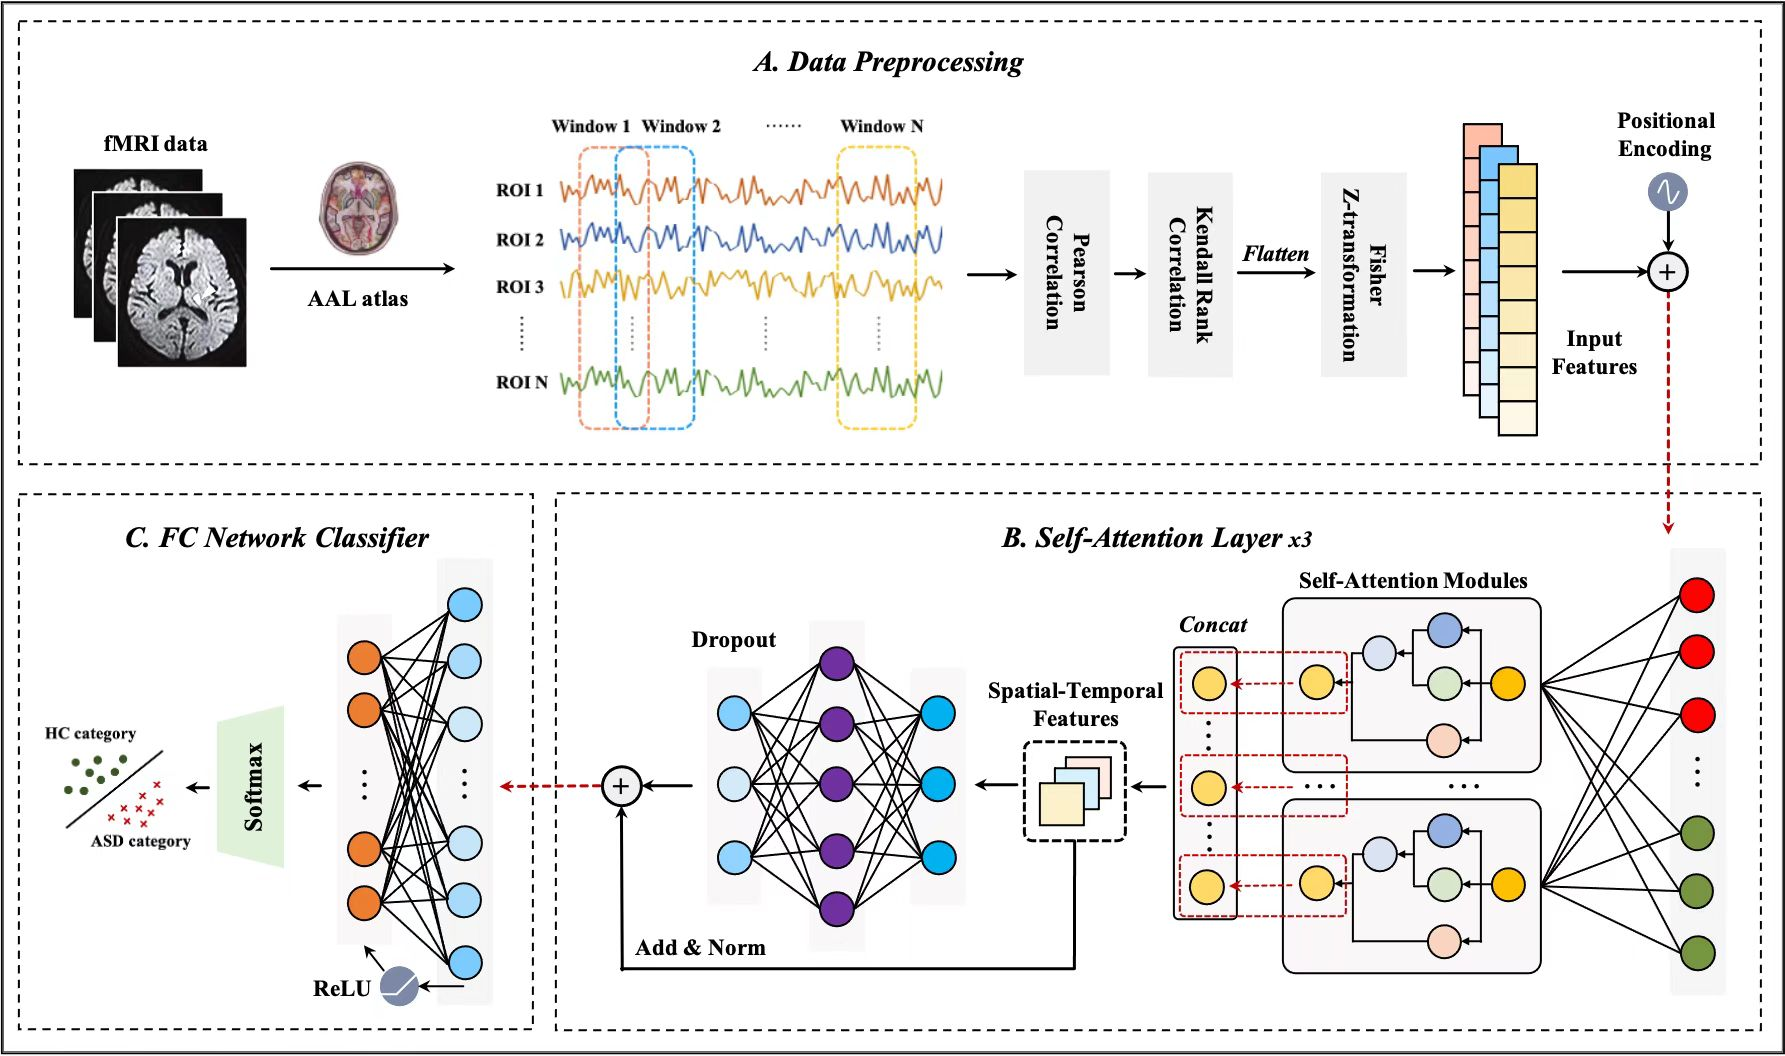
\includegraphics[width=\textwidth]{imgs/model.jpg}
	\caption{Flowchart of the proposed model. Box A shows the acquisition and feature extraction of dynamic functional connections. Box B shows the core model structure based on the self-attention mechanism. Box C shows the result classification based on the fully connected layer}
	\label{fig1}
\end{figure*} 

\subsection{Construction of Brain Functional Network}
The complete flow chart of the model is shown in Fig.\ref{fig1}. This section will explain how to generate dynamic brain functional connectivity networks using preprocessed data. 
%\paragraph{Silding Windows Method}~{}

Initially, assume that a window of fixed length $l$ moves through the time series of data at a constant step $s$. The window partitions the entire time series into many overlapping but mutually distinct subsequences. The sliding window method requires the selection of parameters such as window length and step size beforehand. The window length determines the trade-off between temporal resolution and estimating precision\cite{savva2019assessment}. Smaller window sizes are more sensitive to changes in time, but they add more noise,  which exacerbates the challenges of small sample sizes and high dimensionality. Based on previous research, we set the window length $l$ = 30 and the step size $s$ = 1. We divide the preprocessed data into $N$ separate windows,where $N = \left \lfloor \frac{T - l}{s} \right \rfloor + 1$
%\paragraph{Pearson's Correlation Coefficient}~{}

Brain connections create a sophisticated network that enables a variety of high-level tasks. Pearson's correlation coefficient is widely used to establish functional connectivity between brain regions. It quantifies the linear relationship between two variables, in this case the BOLD signal time series of two brains. When there is a strong linear correlation between two brain regions, it suggests that they are likely involved in a common functional task.\cite{ju2017early}.

Pearson's correlation coefficient assumes that the data follow a normal distribution. To ensure the reliability and interpretability of our correlation analysis, we assessed whether the data followed a normal distribution using the Shapiro-Wilk test on randomly selected brain regions for each sample. The results($P=0.421\pm 0.295>0.05$, $W=0.989\pm 0.004$) indicate that we could not reject the null hypothesis at the 0.05 level of significance, confirming that the time series followed a normal distribution.

For each window $W_n$, we define $x_{i}(t)$ and $x_{j}(t)$ as the BOLD signals of two brain regions $i$ and $j$ at time point $t$($t = 1,2,...,l$).The functional connectivity $FC_{ij}$ between regions $i$ and $j$ can be calculated as,
\begin{equation}
	FC_{ij}=\frac{\sum_{t=1}^{l}(x_{i}(t)-\bar{x_{i}})(x_{j}(t)-\bar{x_{j}})}{\sqrt{\sum_{t=1}^{l}(x_{i}(t)-\bar{x_{i}})^2}\sqrt{\sum_{t=1}^{l}(x_{j}(t)-\bar{x_{j}})^2}}
\end{equation}

where $\bar{x_{i}}$ and $\bar{x_{j}}$ represent the mean of rs-fMRI in brain regions $i$ and $j$. For AAL with 116 ROIs and CC200 with 200 ROIs, the calculation between each pair of regions results in $F$ features, where $F=6670$ for AAL and $F=19900$ for CC200. Each window's feature vector contains all $F$ features and is concatenated to form a sample's feature matrix. The shape of the resulting feature matrix can be expressed as $N\times F$.
\subsection{Feature Ranking by Dynamic Kendall Rank Correlation}
Compared with static FC, dFC providesa more informative representation of brain activity while making the problem of high feature dimensionality more significant. To extract more meaningful information while reducing noise and improving computational efficiency, we employed a feature selection approach based on the Kendall rank correlation coefficient. This metric measures the relevance of each feature to classification by a distribution-free test of independence between two variables\cite{zeng2012identifying}. We apply this method to each window separately and combine the obtained rankings to determine the final set of selected features. 

Assume that $m$ and $n$ correspondingly represent the number of ASD patients group and HC group. For each windows $i$ and feature $j$, we denote $z_{jk}$ as the $j$-th feature of the $k$-th sample, and $y_k$ as its class label. To quantify the discriminative power of feature $j$ in the $i$-th window, we employ the Kendall tau correlation coefficient $\tau_{ij}$, defined as,
\begin{equation}
	\tau_{ij} = \frac{n_c - n_d}{m \times n}
\end{equation}
Here, $n_c$ and $n_d$ represent the numbers of concordant and discordant pairs. between $z_{jp}$ from the ASD patient group ans $z_{jq}$ from the HC group,respectively. We consider a pair as concordant when
\begin{equation}
	sgn(z_{jp} - z_{jq}) = sgn(y_p-y_q)
\end{equation}
where sgn() is a signum function. Correspondingly, it is a disconcordant pair when
\begin{equation}
	sgn(z_{jp} - z_{jq}) = -sgn(y_p-y_q)
\end{equation}

The absolute value of each $\tau_{ij}$ reflects the ability of feature $j$ to detect ASD in the $i$-th window, with a higher absolute value indicating a tronger discriminative power. To represent the combined discriminative capacity of feature $j$ across all windows, we average its correlation coefficients $\tau_{ij}$ over all windows, yielding $\tau_{j}$, which can be expressed as:
\begin{equation}
	\tau_{j} =  \frac{1}{N}\sum_{i=1}^{N}\tau_{ij}
\end{equation}


To identify the most informative features for detecting ASD, we rank the $\tau_{j}$ values in descending order and select the top $C$ ($C\leq F$) features. The value of $C$ is chosen based on the sparsity of functional brain connections, as a smaller $C$ may reduce noise but also risk losing meaningful information. 

Recalling the calculation of features, it actually represents the correlations between the BOLD signals of two brain regions, with higher-ranked features indicating stronger connections between corresponding regions more likely to be associated with ASD.
\subsection{Classification based on Multi-Head Self-Attention}
%\subsubsection{Positional Encoding}
Self-attention mechanisms are useful in helping models understand global relationships between inputs by assigning different weights to input and identifying essential information. However, while its parallelism increases the efficiency of  model operations, it disregards the order of the model's inputs, which means changing the order of the  inputs has no effect on the model's output\cite{litjens2017survey}. It can lead to a loss of temporal information, particularly when the inputs are continuous time windows.

To address this issue, we adopt the position encoding strategy used in  Transformer\cite{vaswani2017attention}, which appends position information to the input data before it enters the self-attention layer. Specifically, for each independent window $n_i(i=1,2,..., N)$ and each feature vector index $c_j(j=1,2..., C)$, we use sine and cosine functions with different frequencies to determine the positional encoding $PE$, defined as,
\begin{equation}
	PE_{(c_i,2k)}=sin(c_i/10000^{2k/C})
\end{equation}
\begin{equation}
	PE_{(c_i,2k)}=cos(c_i/10000^{2k/C})
\end{equation}
Here, $k(k<\frac{j}{2})$ is used to map to index $j$. $PE$ is then added to each sample's data to provide positional encoding information without expanding the data's dimensions.

The self-attention layer is a crucial component of our model, which takes $N$ windows with dimension $C$ as input. The vector $I = (I_0, I_1,..., I_N)$ is first fed into the self-attention layer, where three matrix $Q$, $K$ and $V$ are defined as
\begin{equation}
	Q_i = I W_{Qi}, \quad K_i = I W_{Ki}, \quad V_i = I W_{Vi}
\end{equation}
where $i$ denotes the $i$-th attention head, and $W_{Qi}$, $W_{Ki}$ and $W_{Vi}$ are learnable weight matrices specific to each head. For each head $i$, we compute the attention weights $\alpha_i$ are then defined as
\begin{equation}
	\alpha_i = Softmax(\frac{Q_iK_i^T}{\sqrt{d_k}})
\end{equation}
where $d_k$ is the dimension of the K matrix. The Softmax function is used to normalize the weights so that they sum to 1. Then the output matrix $O_i$ for each head $i$ is defined as
\begin{equation}
	O_i = \alpha_i V_i
\end{equation}

Figure.\ref{fig2} shows the schematic diagram of the self-attention mechanism.  Due to the complexity of brain functional connectivity, we employed a multi-head self-attention layer to obtain rich information on functional connectivity. The multi-head self-attention layer creates $H$ subspaces, executes the self-attention function on each subspace in parallel, and then concatenate the output matrices of all heads on temporal dimension to obtain the final output matrix $O$, which can be represented as,
\begin{equation}
	O = Concatenate(O_1, O_2,..., O_H)
\end{equation}
where $Concatenate$ is the concatenation operation.

To extract higher-order features while reducing the number of parameters, we stacked multiple layers of the multi-head self-attention layer. Specifically, we made the dimension $d_v$ of the matrix $V$ smaller than the dimension $d_{qk}$ of matrices $Q$ and $K$ for dimensionality reduction. The output dimension of the multi-head self-attention layer can be expressed as $N\times Hd_v$. With the structure, the model can extract more discriminative spatial features while capturing temporal correlations between windows. In this experiment, we stacked three layers of multi-head self-attention layers, with the number of features per window for each output layer being 500, 200, and 50.

\begin{figure}[htb]
	\centering
	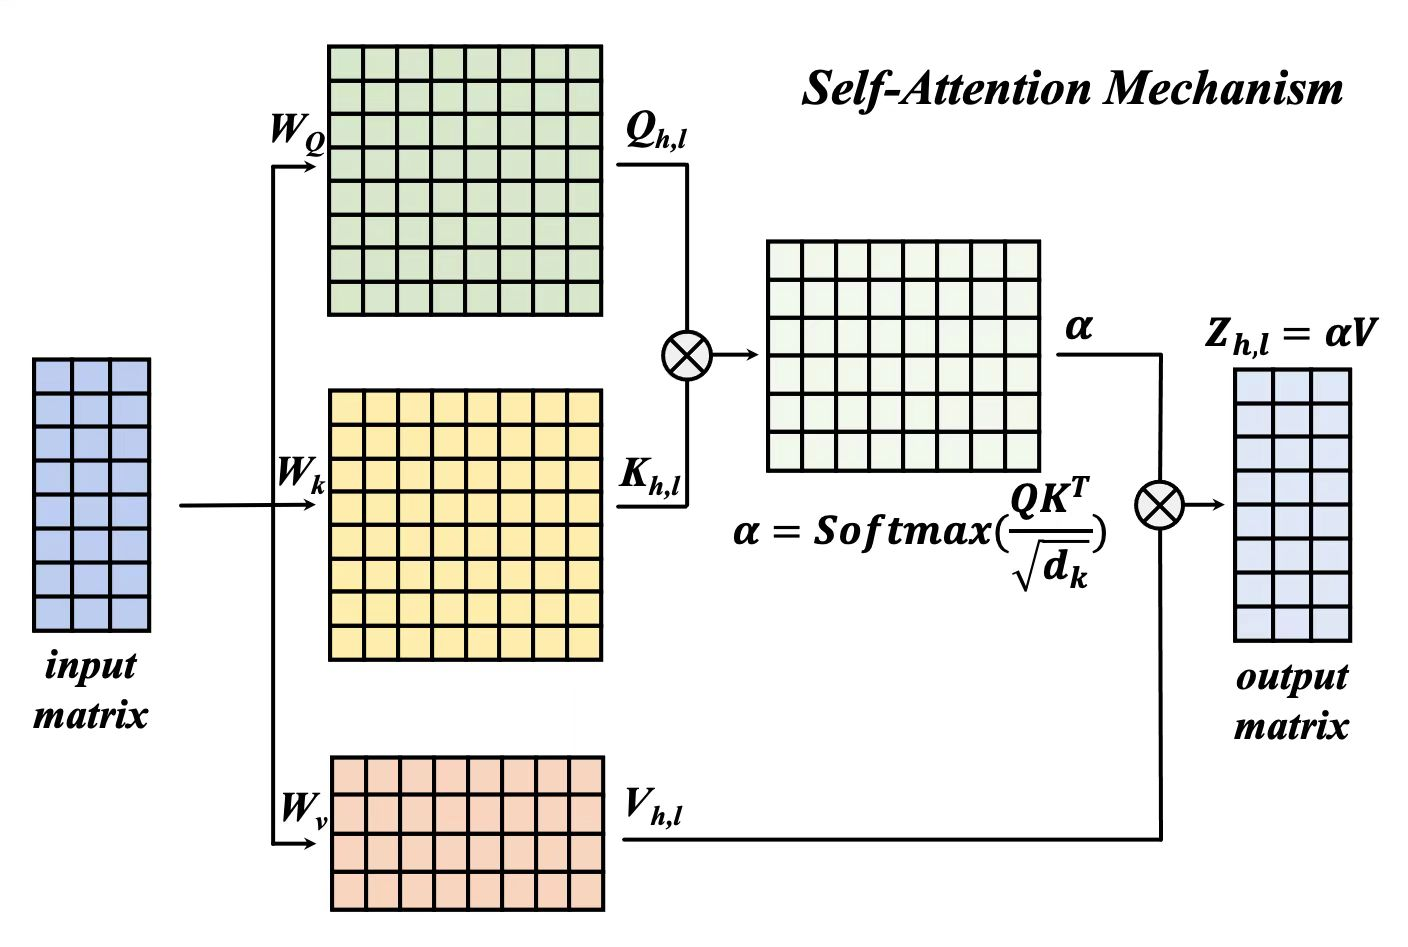
\includegraphics[width=0.48\textwidth]{imgs/attention.jpg}
	\caption{Self-Attention Mechanism Structure}
	\label{fig2}
\end{figure} 

We incorporated feedforward neural networks between the multi-head self-attention layers to achieve nonlinear transformation of features. Specifically, we used a linear projection layer to transfer the output of the self-attention layer to a high dimension, followed by a ReLU activation function to combine features and produce deeper associations. Then, another linear projection layer was used to reduce the higher-dimensional output back to the original dimension, eliminating combinations with low discriminatory power. To avoid the gradient vanishing and speed up the model's training, we added a residual network to the feedforward neural network. This feedforward neural network can be represented as,
\begin{equation}
	FFN(X) = ReLU(XW_1)W_2 + X
\end{equation}
where $W_1$ and $W_2$ are learnable weight matrices.

Additionally, we utilized a Dropout layer to prevent overfitting of the model. The flow chart of the algorithm is shown in Algorithm I.

Following these operations, the data was reduced to two dimensions by the fully connected layer, and the model output was generated by Softmax. We used the cross-entropy loss function combined with the L2 regularized loss function as our loss function, which can be represented as,
\begin{equation}
	L = -\frac{1}{N}\sum_{i=1}^{N}\sum_{j=1}^{C}y_{ij}\log(p_{ij}) + \lambda||\theta||_2^2
\end{equation}
where $p_{ij}$ represents the predicted probability of class $j$ for sample i, $\lambda$ is the regularization coefficient, which is set to 0.0001, and $\theta$ denotes the model parameters. The optimizer used was SGD.
\begin{table}
	\centering
	%\refstepcounter{table}
	\begin{tabular}{>{\hspace{0pt}}m{0.933\linewidth}} 
		\toprule
		\textbf{Algorithm 1} Multi-Head Self-Attention Based DNN Model                   \\ 
		\midrule
		\textbf{Input}: Input matrix $I$                                         \\
		\textbf{Output}: Result probability $O$                                  \\
		Initialization: learnable weight matrix $W_Q$, $W_K$, $W_V$, $W_1$, $W_2$, $W$                        \\
		hyperparameters: $H$,$d_k$,$d_v$,$max\_layer$                            \\
		1: ~~\textbf{while} epoch \textless{} max\_epochs \textbf{do}            \\
		2: ~~ \quad \textbf{for} $l \leftarrow 1$ \textbf{to} max\_layers \textbf{do}  \\
		3: ~~ \qquad \textbf{for} $i \leftarrow 1$ \textbf{to} $H$ \textbf{do}          \\
		4:  ~~ \qquad \quad calculate the output of each head                                \\
		\textcolor{white}{4:} ~~ \qquad \quad $Q_{i,l}=IW_{Qi}$,$K_{i,l}=IW_{Ki}$,$V_{h,l}=IW_{Vi}$          \\
		5: ~~ \qquad \quad $\alpha_i = Softmax(Q_iK_i^T / \sqrt{d_k})$                              \\
		6: ~~ \qquad \quad $Z_{i,l} = \alpha V_i$                                                 \\
		7: ~~ \qquad \textbf{end for}                                                   \\
		8:  ~~ \qquad Merge the results of each head                                    \\
		\textcolor{white}{8:} ~~ \qquad $Z_l = Concatenate(Z_{1,l},Z_{2,l},...,Z_{h,l})$      \\
		9: ~~ \qquad Feedforward and residual networks	\\
		\textcolor{white}{9: ~~} \qquad $U_l = ReLU(Z_lW_{1,l})W_{2,l} + Z_l$                                             \\                     
		10: ~~\qquad $I\leftarrow H_l$                                                    \\
		11:~~ \quad \textbf{end for}                                                     \\
		12:~~ \quad$O = Softmax(WH_l)$                                                   \\
		13:~~ \quad \textbf{update network}                                              \\
		14:~~ \quad \textbf{end while}                                                    \\
		15:~~ return $O$                                                              \\
		\bottomrule
	\end{tabular}
\end{table}


\section{Result}
In this section, we analyze the effect of the number of chosen features and the number of heads of the multi-head self-attention layers, compare our method  to previous models, and demonstrate the brain region connections most likely to induce ASD.
\subsection{Impact of feature numbers and head numbers to classification results}
Due to the sparsity of brain connections and the high dimensionality, the number of features chosen becomes a key determinant of classification outcomes. To determine the optimal value for the number of features, we trained the model using the top 100, 512, 1024, 1600, and 6670 Kendall features, respectively, and chose accuracy, sensitivity, specificity and AUC as evaluation indicators. The conclusive results are shown in Table \ref{Table2}. 

We observed that the model performs best with 1024 features using AAL and 800 features using CC200, indicating the presence of significant noise in the raw data and the importance of feature extraction. To demonstrate the reliability of feature ranking, we randomly picked 1024 features using AAL for testing, and the results verified that Kendall can not only reduces data dimensionality but also effectively selects the most discriminative features.
\begin{table*}
	\centering
	\caption{Experimental results using 100, 512, 1024, 1600, and 6670 features as model inputs,(r) means random}
	\label{Table2}
	\tabcolsep=1cm
	\begin{tabular*}{\textwidth}{cccccc}
		\toprule
		\multicolumn{1}{l}{\textbf{Template}} & \textbf{Number} & \textbf{Accuracy}  & \textbf{Sensitivity}  & \textbf{Specificity}  & \textbf{AUC}      \\ 
		\midrule
		\multirow{7}{*}{AAL}                  & 100             & 0.7090             & 0.6453                & 0.7651                & 0.7664            \\
		& 512             & 0.7448             & \textbf{0.7112}       & 0.7759                & 0.8080            \\
		& 800             & 0.7566             & 0.6343                & 0.8577                & 0.7933            \\
		& 1024            & \textbf{0.7622}    & 0.6554                & 0.8458                & \textbf{0.8132}   \\
		& 1024(r)         & 0.6045             & 0.2869                & 0.8426                & 0.6162            \\
		& 1600            & 0.7463             & 0.6253                & 0.8490                & 0.7930            \\
		& 6670            & 0.6716             & 0.4482                & \textbf{0.8583}       & 0.7034            \\ 
		\midrule
		\multirow{6}{*}{CC200}                & 100             & 0.7300             & 0.5956                & 0.8369                & 0.7647            \\
		& 512             & 0.7783             & 0.7280                & 0.8159                & 0.8182            \\
		& 800             & \textbf{0.7965}    & \textbf{0.7660}       & 0.8190                & \textbf{0.8221}   \\
		& 1024            & 0.7819             & 0.7231                & 0.8382                & 0.8133            \\
		& 1600            & 0.7744             & 0.7384                & 0.8088                & 0.8217            \\
		& 6670            & 0.7707             & 0.6740                & \textbf{0.8462}       & 0.8134            \\
		\bottomrule
	\end{tabular*}
\end{table*}

We also investigated the effect of the number of heads $H$ on model performance in the multi-head self-attention layers, and the experimental results are shown in Table \ref{Table3}. The model performed best at $H$ = 6, indicating that functional brain connections contain a wealth of information that can be effectively captured by the multi-head self-attention layer. However, when the number of heads exceeds six, it becomes increasingly difficult for the number of samples to support the training of a high number of parameters, resulting in a decline in the model's efficacy.
\begin{table*}
	\centering
	\caption{Experimental results using 1,2,4,6,8 heads in multi-head self-attention layers}
	\label{Table3}
	\tabcolsep=1cm
	\begin{tabular*}{\textwidth}{cccccc}
		\toprule
		\multicolumn{1}{l}{\textbf{Template}} & \textbf{Number} & \textbf{Accuracy} & \textbf{Sensitivity} & \textbf{Specificity} & \textbf{AUC}     \\ 
		\midrule
		\multirow{5}{*}{AAL}                  & 1               & 0.7343            & 0.6465               & 0.8123               & 0.7996           \\
		& 2               & 0.7507            & \textbf{0.6751}      & 0.8177               & 0.8022           \\
		& 4               & 0.7358            & 0.6190               & 0.8315               & 0.8028           \\
		& 6               & \textbf{0.7622}   & 0.6554               & \textbf{0.8458}      & \textbf{0.8132}  \\
		& 8               & 0.7343            & 0.6039               & 0.8451               & 0.8040           \\ 
		\midrule
		\multirow{5}{*}{CC200}                & 1               & 0.7587            & 0.6661               & 0.8328               & 0.8031           \\
		& 2               & 0.7708            & 0.7246               & 0.8046               & 0.8157           \\
		& 4               & 0.7895            & 0.7846               & 0.7941               & 0.8104           \\
		& 6               & \textbf{0.7965}   & 0.7660               & \textbf{0.8190}      & 0.8221           \\
		& 8               & 0.7895            & \textbf{0.8036}      & 0.7792               & \textbf{0.8381}  \\
		\bottomrule
	\end{tabular*}
\end{table*}

\subsection{Results presentation and model comparison}
We employed the k-fold cross-validation method to maximize the use of samples for model testing, which is commonly employed on small sample datasets. Specifically, we divide all samples into $k$ equal-sized folds, and repeats this process $k$ times, each time using a different fold as the test set and the remaining folds as the training set. In this paper we selected $k=10$ for the cross-validation procedure.

We applied multiple models for comparison. The first model applied was a logistic regression (LR) with L2 regularization terms and 1000 maximum iterations. Then, a support vector machine based on the rbf kernel function was constructed with the penalty value set to 1. Both LR and SVM were applied using dFC data, and Kendall rank correlation coefficients were used for feature extraction.

We have also implemented the four deep learning algorithms listed below. First, a fully connected neural network reduces the spatial dimension from 1024 to 400, 100, and 50 before splicing and flattening it in the temporal dimension and finally reducing it to two dimensions. Second, a model that gradually extracts high-level features by stacking 3D-CNNs, employing ELU activation functions and L2 regular terms with a value of 0.005 was applied\cite{deng2022diagnosing}. Third, a model that imitates the LSTM model and employs a two-layer LSTM to extract information from time series following feature extraction\cite{dvornek2017identifying}. Finally, we applied a model that employs CNN for feature extraction, LSTM for temporal information extraction, a single self-attention layer for higher-order feature extraction, and a fully connected layer for classification\cite{xu2021identification}.

The results are shown in Table \ref{Table4}. The ROC curves for all models are shown in Fig.\ref{fig3}. The CC20 template-based model proposed in this paper achieves an average accuracy of 79.65\% in ten folds, with better sensitivity and AUC compared to similar models, which indicates that our model has excellent classification performance. 

\begin{table*}[]
	\centering
	\caption{Comparison of the classification performances between our method and other methods}\label{Table4}
	\tabcolsep=0.95cm
	\begin{tabular*}{\textwidth}{cccccc}
		\toprule
		\multicolumn{1}{l}{\textbf{Template}} & \textbf{Model} & \textbf{Accuracy}         & \textbf{Sensitivity}      & \textbf{Specificity} & \textbf{AUC}               \\ 
		\midrule
		\multirow{7}{*}{AAL}                  & LR             & 0.7272                    & 0.6723                    & 0.7771               & 0.7245                     \\
		& SVM            & 0.7404                    & 0.6134                    & \textbf{0.8514}      & 0.7322                     \\
		& FC             & 0.7537                    & 0.6890                    & 0.8053               & 0.7954                     \\
		& CNN            & 0.6836                    & 0.5847                    & 0.7628               & 0.6207                     \\
		& LSTM           & 0.7164                    & 0.5966                    & 0.8151               & 0.7619                     \\
		& CLAttention    & 0.7448                    & 0.6369                    & 0.8356               & 0.7990                     \\
		& our method     & \textbf{\textbf{0.7622}}  & \textbf{\textbf{0.6554}}  & 0.8458               & \textbf{\textbf{0.8132}}   \\ 
		\midrule
		\multirow{7}{*}{CC200}                & LR             & 0.7330                    & 0.6880                    & 0.7708               & 0.8134                     \\
		& SVM            & 0.7452                    & 0.6719                    & 0.8064               & 0.8215                     \\
		& FC             & 0.7737                    & 0.7120                    & 0.8176               & 0.8154                     \\
		& CNN            & 0.6652                    & 0.5709                    & 0.7423               & 0.6818                     \\
		& LSTM           & 0.7210                    & 0.6003                    & 0.8153               & 0.7612                     \\
		& CLAttention    & 0.7436                    & 0.6092                    & \textbf{0.8528}      & 0.7941                     \\
		& our method     & \textbf{0.7965}           & \textbf{0.7660}           & 0.8190               & \textbf{0.8221}           \\
		\bottomrule
	\end{tabular*}
\end{table*}

\begin{figure}[htb]
	\centering
	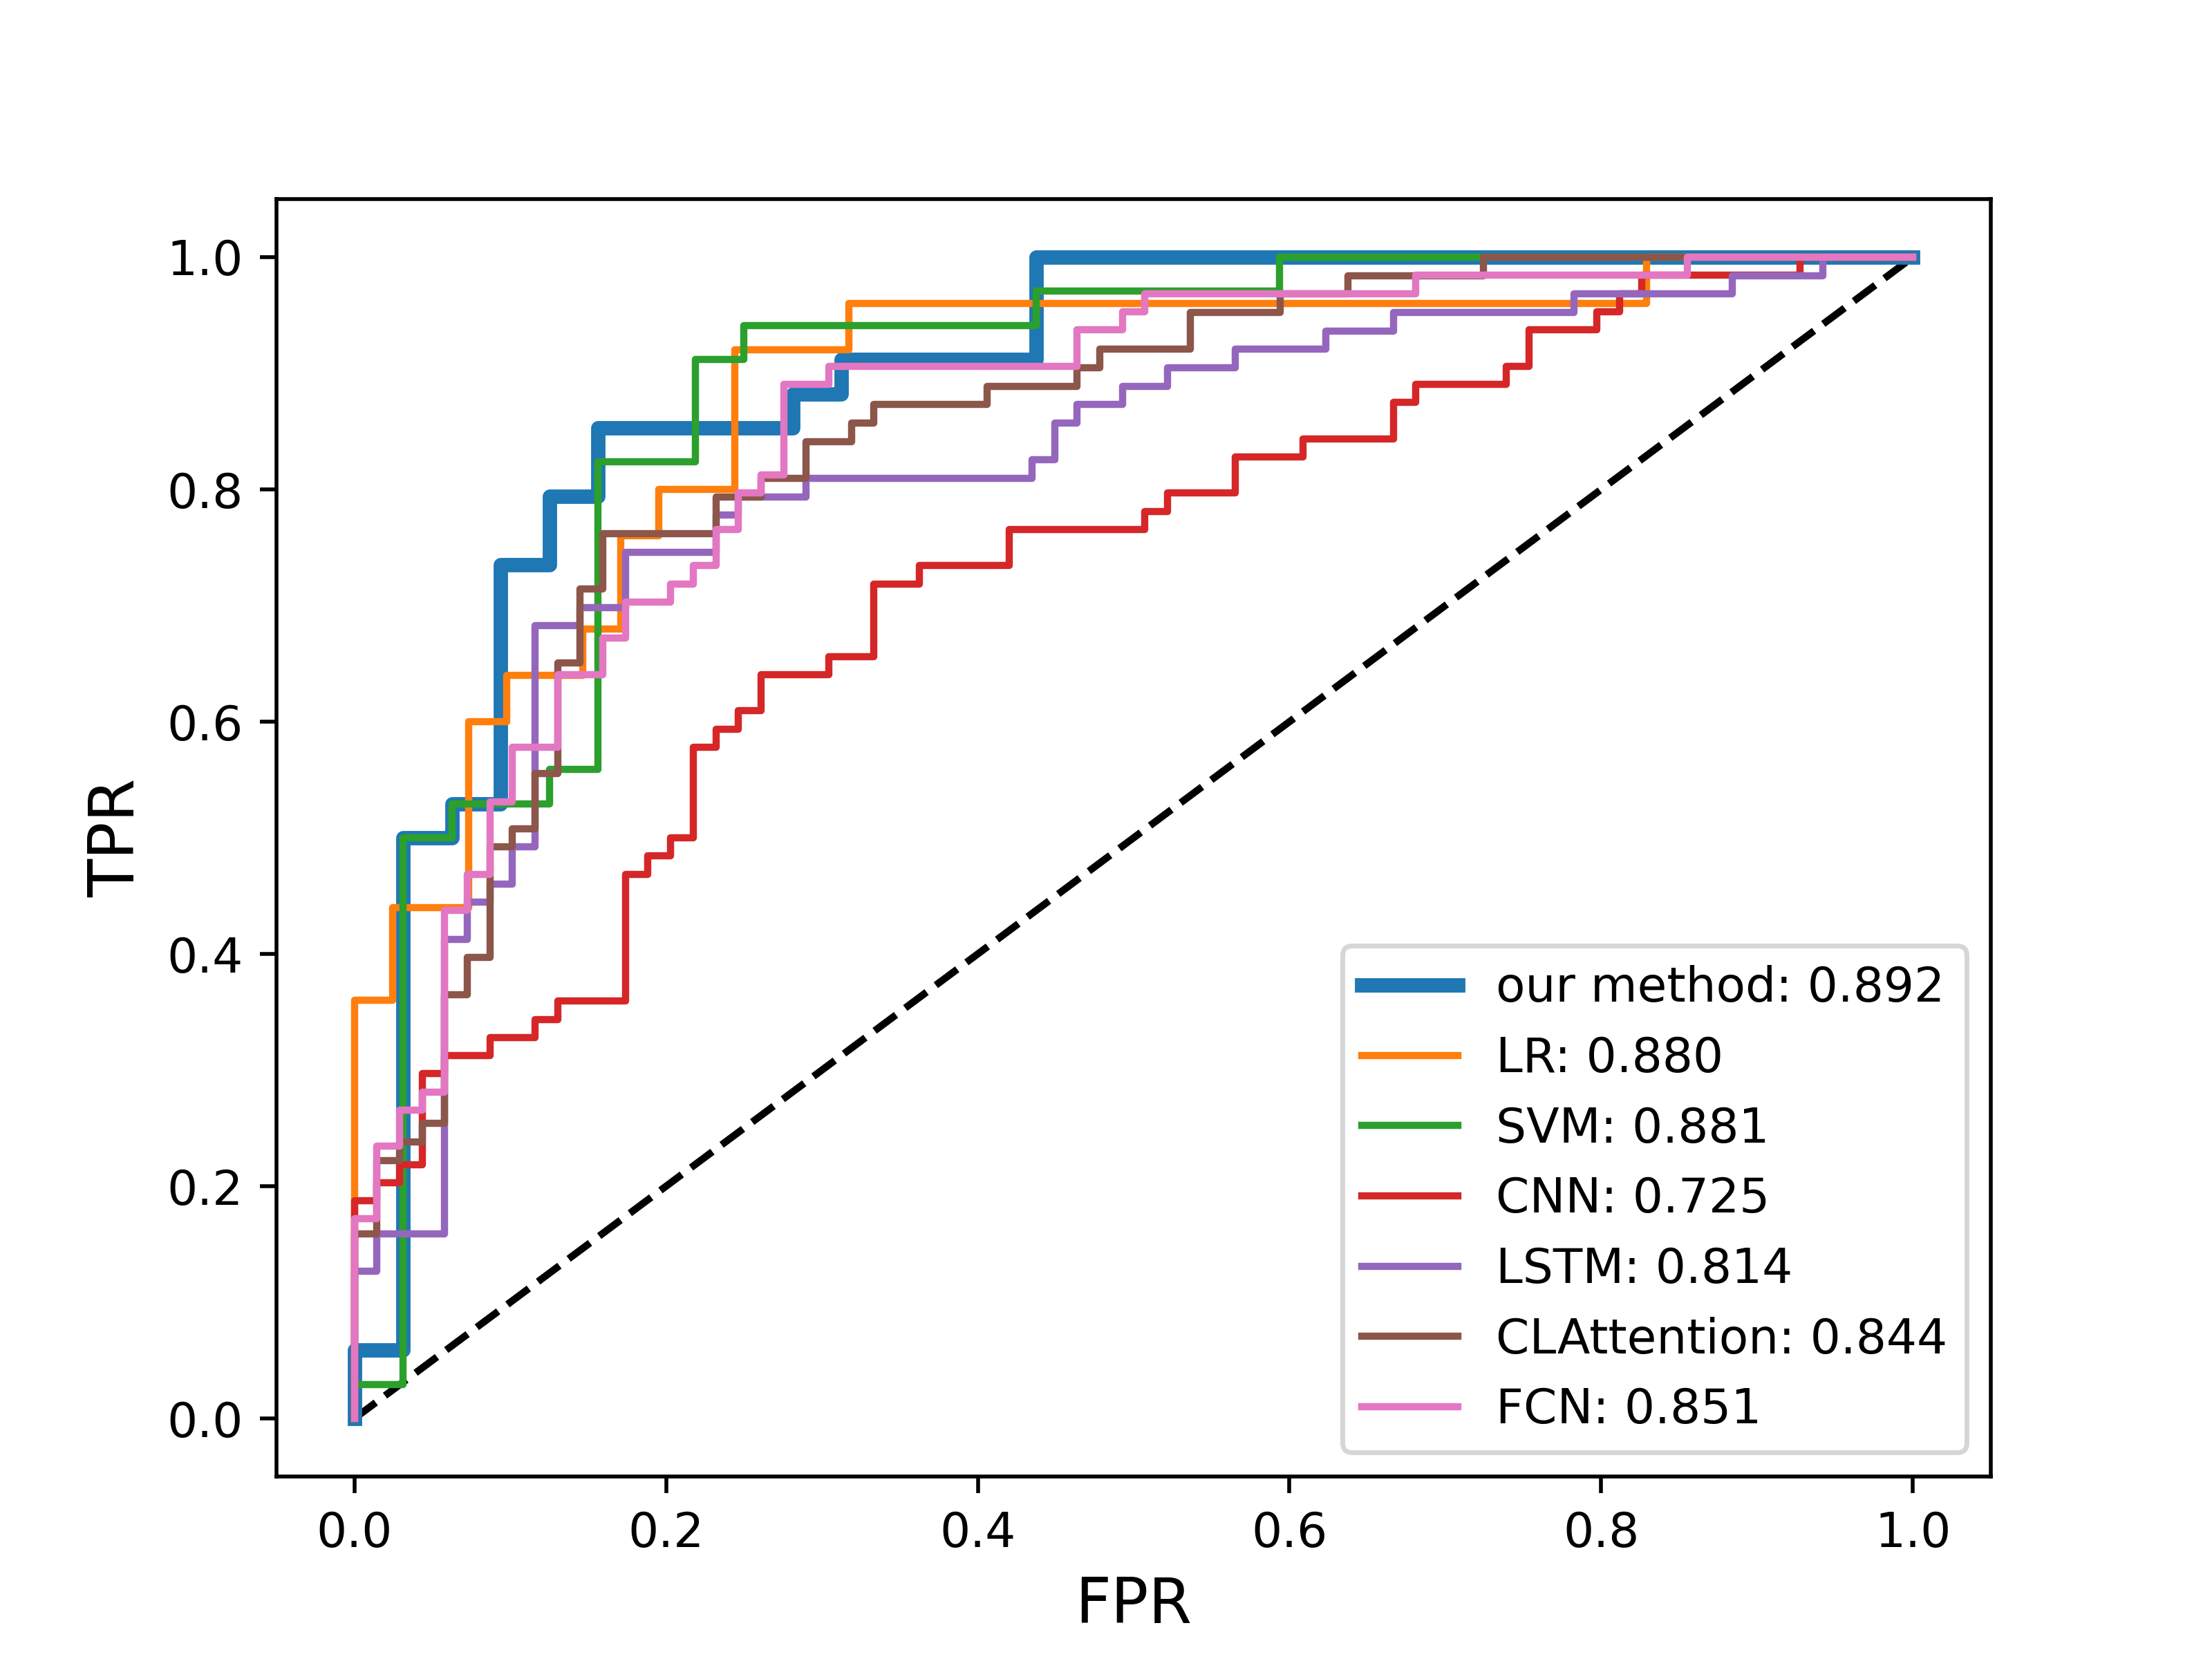
\includegraphics[width=0.5\textwidth]{imgs/roc.png}
	\caption{All model's ROC curves}
	\label{fig3}
\end{figure} 
To evaluate the model's generalization ability, we employed inter-site cross-validation, where one site's samples were used as the test set, and the other sites' samples were used as the training set. This approach was necessary to account for inherent challenges in achieving uniformity in data acquisition and processing across different sites\cite{ingalhalikar2021functional}. We selected eight sites with sample sizes greater than 5\% of the total sample size to ensure the robustness of our findings. The results, presented in Table \ref{Table5}, demonstrate that our model achieved an average accuracy of 76.71\% with AAL and 78.47\% with CC200 across all sites, indicating exceptional generalizability.

\begin{table*}
	\centering
	\caption{Experimental results on sites with over 5\% of the sample size}
	\label{Table5}
	\tabcolsep=0.8cm
	\begin{tabular*}{\textwidth}{ccccccc} 
		\toprule
		\multicolumn{1}{l}{\textbf{Template}} & \textbf{Sites} & \textbf{Size} & \textbf{Accuracy} & \textbf{Sensitivity} & \textbf{Specificity} & \textbf{AUC}  \\ 
		\midrule
		\multirow{9}{*}{AAL}                  & KKI            & 34            & 0.7353            & 0.5000               & 0.7500               & 0.6625        \\
		& LEUVEN         & 60            & 0.7167            & 0.4074               & 0.9697               & 0.7991        \\
		& NYU            & 166           & 0.7470            & 0.7042               & 0.7789               & 0.7732        \\
		& STANFORD       & 36            & 0.6667            & 0.8235               & 0.5263               & 0.6873        \\
		& TRINITY        & 43            & 0.7857            & 0.7619               & 0.8095               & 0.8662        \\
		& UM             & 113           & 0.7857            & 0.7659               & 0.8000               & 0.8245        \\
		& USM            & 61            & 0.7833            & 0.7027               & 0.9130               & 0.8409        \\
		& YALE           & 48            & 0.9167            & 0.9545               & 0.8846               & 0.9126        \\ 

		& AVG            & 70            & 0.7671            & 0.7025               & 0.8040               & 0.7958        \\ 
		\midrule
		\multirow{9}{*}{CC200}                & KKI            & 34            & 0.7647            & 0.5000               & 0.8750               & 0.7667        \\
		& LEUVEN         & 60            & 0.7333            & 0.3846               & 1.0000               & 0.8389        \\
		& NYU            & 166           & 0.7651            & 0.7714               & 0.7553               & 0.8051        \\
		& STANFORD       & 36            & 0.6389            & 0.8824               & 0.4211               & 0.6687        \\
		& TRINITY        & 43            & 0.7674            & 0.7500               & 0.8000               & 0.7975        \\
		& UM             & 113           & 0.8318            & 0.8085               & 0.8308               & 0.8858        \\
		& USM            & 61            & 0.9016            & 0.8684               & 0.9545               & 0.9043        \\
		& YALE           & 48            & 0.8749            & 0.7143               & 1.0000               & 0.9200        \\ 
		& AVG            & 70            & 0.7847            & 0.7100               & 0.8296               & 0.8234        \\
		\bottomrule
	\end{tabular*}
\end{table*}

\subsection{Functional connections that may lead to ASD}
In our previous work, we ranked the features for all $N$ windows using the Kendall rank correlation coefficient, where features with higher rankings were considered to be more discriminatory. The construction process of features quantified the degree of correlation between two distinct brain regions. Therefore, features with higher rankings indicated a stronger correlation between the brain regions are more likely to be associated with ASD.

\begin{figure*}[h]
	\centering
	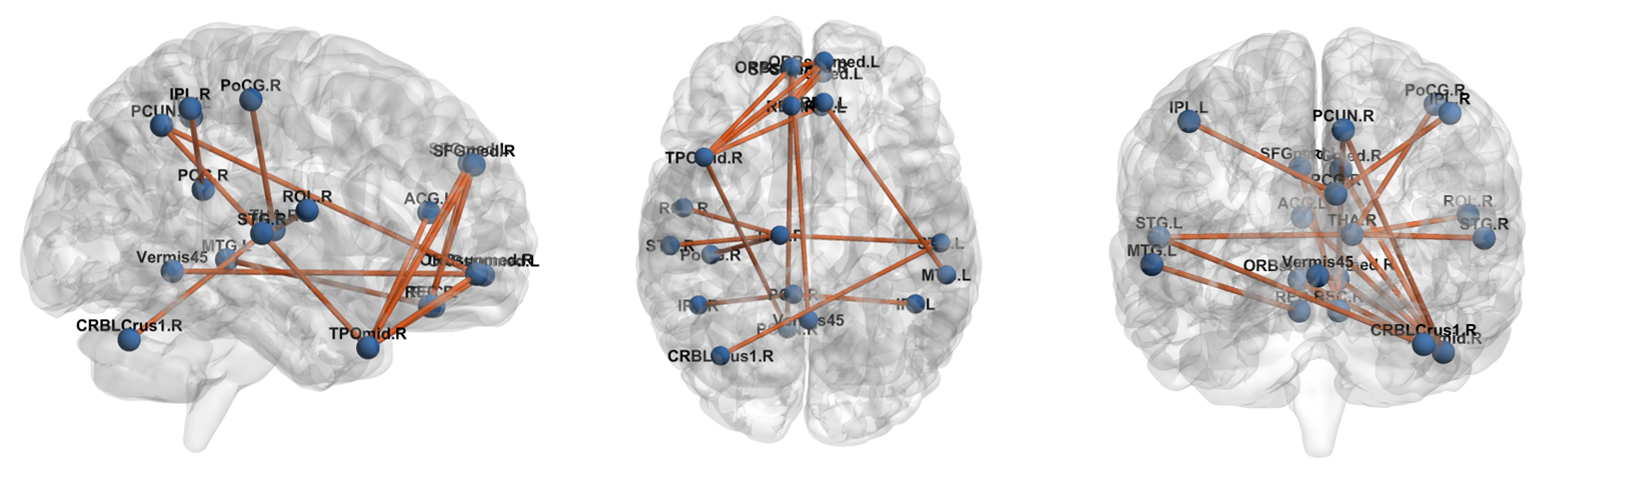
\includegraphics[width=\textwidth]{imgs/brain4.png}
	\caption{Projection of the top 20 most discriminative functional connections in the brain}
	\label{fig4}
	
\end{figure*} 

\begin{figure}[h]
	\centering
	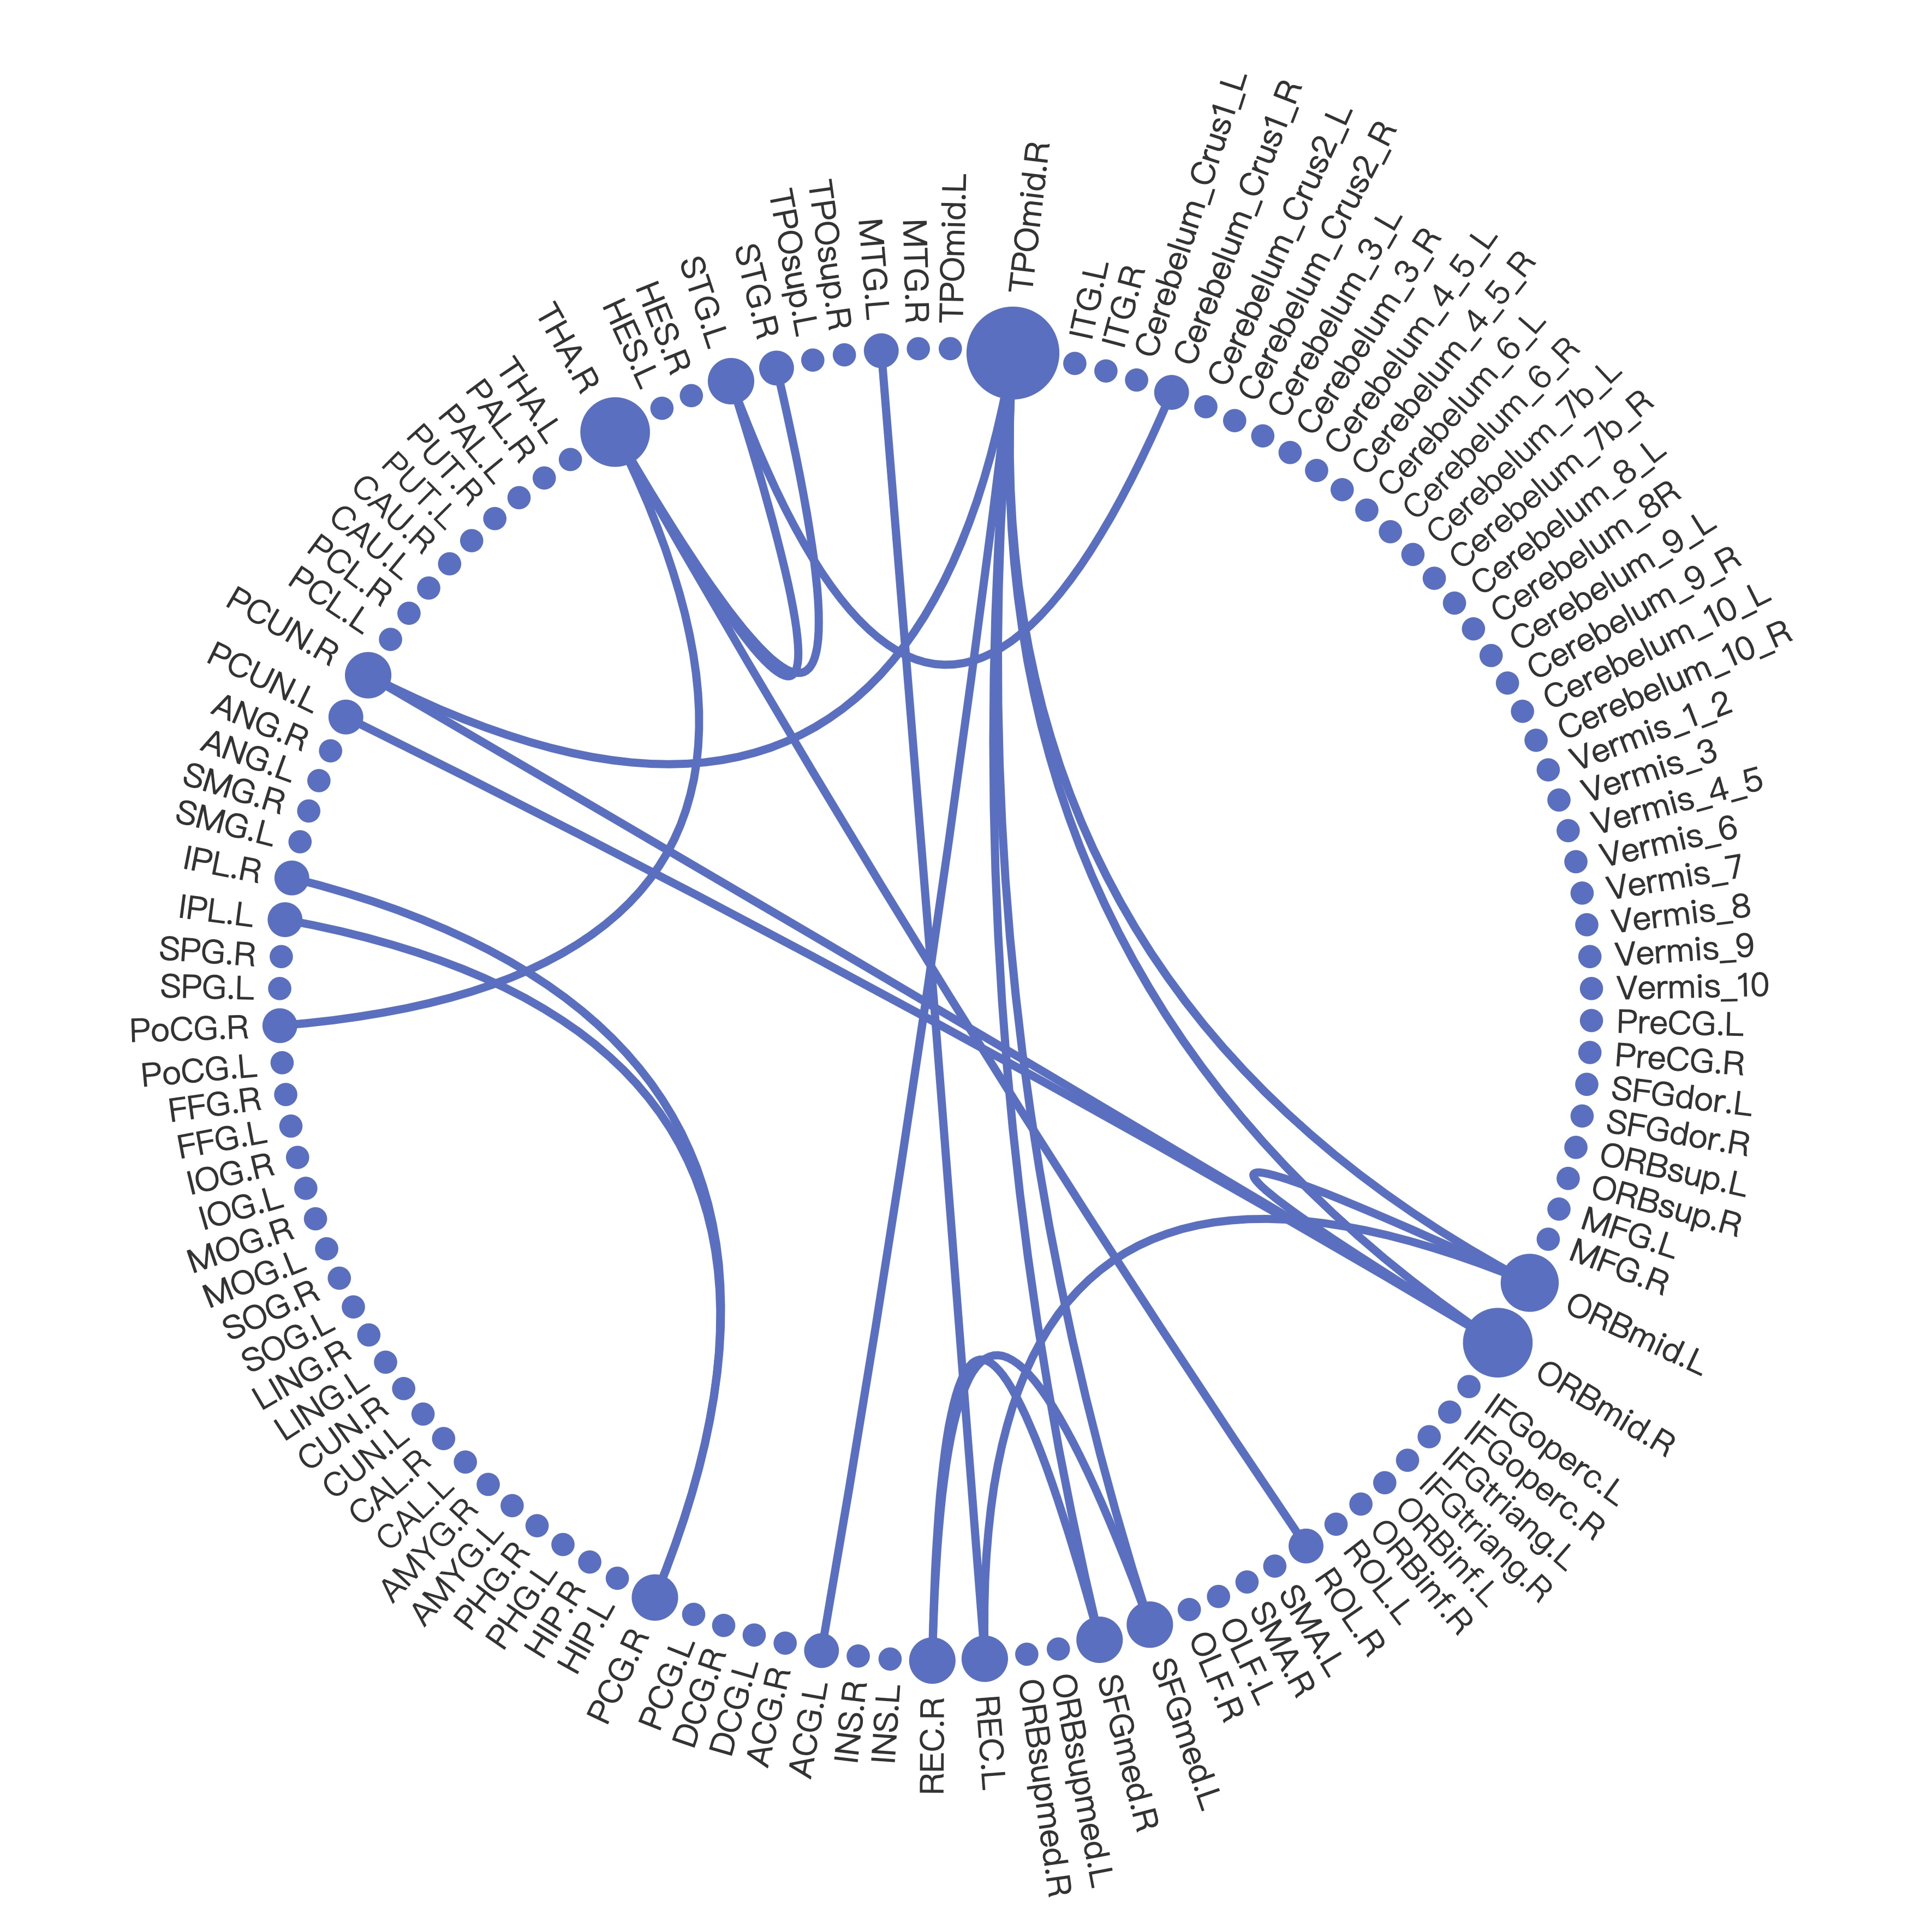
\includegraphics[width=0.45\textwidth]{imgs/circus.jpg}
	\caption{Hierarchical edge bundling of the top 20 most discriminative functional connections in the brain}
	\label{fig5}
\end{figure} 


To identify the most relevant features associated with the onset of ASD, we ranked the top 100 features for each window using the Kendall rank correlation coefficient. We tallied the number of times each feature appeared across all rankings and selected the 30 features with the highest number of occurrences for further analysis. The MNI coordinates, hemisphere, and the center of the corresponding brain regions are summarized in Table\ref{Table6}, the brain projection map is depicted in Fig.\ref{fig4} and the hierarchical edge bundling is shown in Fig.\ref{fig5}.

We present our findings in terms of the functional connections that occur most in the top 100, as well as the brain regions that are most commonly observed.  Regarding functional connectivity, the Cingulum Ant(L) and TemporaI Pole Mid(R) were the only functional connections that appeared in all $T$ windows. Connections between Frontal Mid Orb(R) and Precuneus(R), as well as Frontal Sup Medial(L) and Rectus(R), were present in almost all windows. In terms of brain regions, we found that the middle frontal gyrus and middle temporal gyrus have a significant impact on ASD, which is consistent with previous results\cite{wang2021autistic, monk2009abnormalities, xu2020specific, foti2019observational}.

\begin{table*}
	\centering
	\caption{20 brain connections most likely to cause ASD}
	\label{Table6}
	\tabcolsep=0.45cm
	\begin{tabular*}{\textwidth}{ccccccccc} 
		\toprule
		\multirow{2}{*}{\textbf{ID}} & \multirow{2}{*}{\textbf{ROIs(Hemisphere)}} & \multicolumn{3}{c}{\textbf{\textbf{Coordinates(mm)}}} & \multirow{2}{*}{\textbf{\textbf{ROIs(Hemisphere)}}} & \multicolumn{3}{c}{\textbf{\textbf{\textbf{\textbf{Coordinates}}}}}  \\ 
		\cline{3-5}\cline{7-9}
		&                                            & x      & y      & z                                   &                                                     & x      & y      & z                                                  \\ 
		\midrule
		1                            & Cingulum Ant(L)                            & -4.04  & 35.40  & 13.95                               & Temporal Pole Mid(R)                                & 44.22  & 14.55  & -32.23                                             \\
		2                            & Frontal Mid Orb(R)                         & 8.16   & 51.67  & -7.13                               & Precuneus(R)                                        & 9.98   & -56.05 & 43.77                                              \\
		3                            & Frontal Sup MediaI(L)                      & -4.80  & 49.17  & 30.89                               & Rectus(R)                                           & 8.35   & 35.64  & -18.04                                             \\
		4                            & Postcentral(R)                             & 41.43  & -25.49 & 52.55                               & Thalamus(R)                                         & 13.00  & -17.55 & 8.09                                               \\
		5                            & Temporal Sup(L)                            & -53.16 & -20.68 & 7.13                                & Thalamus(R)                                         & 13.00  & -17.55 & 8.09                                               \\
		6                            & Frontal Mid Orb(L)                         & 8.16   & 51.67  & -7.13                               & Frontal Mid Orb(R)                                  & 8.16   & 51.67  & -7.13                                              \\
		7                            & Frontal Sup Medial(R)                      & 9.10   & 50.84  & 30.22                               & Rectus(R)                                           & 8.35   & 35.64  & -18.04                                             \\
		8                            & Frontal Sup Medial(R)                      & 9.10   & 50.84  & 30.22                               & Temporal Pole Mid(R)                                & 44.22  & 14.55  & -32.23                                             \\
		9                            & Thalamus(R)                                & 13.00  & -17.55 & 8.09                                & TemporaI Sup(R)                                     & 58.15  & -21.78 & 6.80                                               \\
		10                           & Frontal Sup Medial(L)                      & -4.80  & 49.17  & 30.89                               & Temporal PoIe Mid(R)                                & 44.22  & 14.55  & -32.23                                             \\
		11                           & Frontal Mid Orb(L)                         & 8.16   & 51.67  & -7.13                               & Rectus(R)                                           & 8.35   & 35.64  & -18.04                                             \\
		12                           & Rolandic Oper(R)                           & 52.65  & -6.25  & 14.63                               & Thalamus(R)                                         & 13.00  & -17.55 & 8.09                                               \\
		13                           & Frontal Mid Orb(R)                         & 33.18  & 52.59  & -10.73                              & Temporal Pole Mid(R)                                & 44.22  & 14.55  & -32.23                                             \\
		14                           & Rectus(L)                                  & -5.08  & 37.03  & -18.14                              & Temporal Mid(L)                                     & -55.52 & -33.80 & -2.20                                              \\
		15                           & Precuneus(R)                               & 9.98   & 37.07  & -18.14                              & Temporal PoIe Mid(R)                                & 44.22  & 14.55  & -32.23                                             \\
		16                           & Cingulum Post(R)                           & 7.44   & -41.81 & 21.87                               & Parietal Inf(R)                                     & 46.46  & -46.29 & 49.54                                              \\
		17                           & Frontal Mid Orb(L)                         & 8.16   & 51.67  & -7.13                               & Temporal PoIe Mid(R)                                & 44.22  & 14.55  & -32.23                                             \\
		18                           & Temporal Sup(L)                           & -53.16 & -20.68 & 7.13                                & Cerebelum Crus 1(R)                                 & 37.46  & -67.14 & -29.55                                             \\
		19                           & Parietal Inf(L)                            & -42.80 & -45.82 & 46.74                               & Cingulum Post(R)                                    & 7.44   & -41.81 & 21.87                                              \\
		20                           & Precuneus(L)                               & -7.24  & 56.07  & 48.01                               & Frontal Mid Orb(R)                                  & 33.18  & 52.59  & -10.73                                             \\
		\bottomrule
	\end{tabular*}
\end{table*}
\vspace{0.1cm}
\section{Discussion}
In this study, we divided the time series into multiple overlapping and independent windows using sliding windows. Using the Pearson correlation coefficient, we generated a functional connectivity vector for each window, which were then combined to generate the dFC matrix. Compared to the commonly used static FC, dFC can capture fluctuations in the temporal dimension of the BOLD signal. However, it also exacerbates the conflict between small sample size and high dimensionality, making feature extraction crucial to similar research.

To select features with high discriminative power without altering the raw data, we employed Kendall's rank correlation coefficient for feature extraction. All feature selection was performed before model training, significantly reducing the time required for training. Our results demonstrated that the model achieved the highest performance when 1024 features are chosen for training for AAL and 800 features for CC200, highlighting the sparsity of the brain functional connectivity network and emphasizing the importance of feature extraction in relevant research. Selecting more discriminative features is a crucial prerequisite for achieving excellent model performance.

To address the self-attention mechanism's inability to account for temporal order, we incorporated positional encoding into the input data. This encoding method accurately represents the input order of the windows without increasing the model's parameters, making it easier for the model to capture variations in nearby windows. The multi-head self-attention mechanism is exceptional at gaining global correlation, with the multiple heads enabling the model to learn from multiple subspaces. In our studies, the model worked optimally at $H$=6, demonstrating that the brain functional connectivity network includes a plethora of information. Future studies should focus on extracting this abundant information, such as utilizing Ho-FCN framework to group FC time series into different clusters, and compute multi-order centroid sequences for each cluster's FC time series to reveal the high-order FC relationships among multiple ROIs\cite{zhao2021constructing}.

We also incorporated feedforward neural networks to obtain feature combinations in higher-dimensional spaces and eliminate feature combinations with low discrimination by recovering the preceding dimension. Additionally, residual networks were used to reduce gradient disappearance and accelerate model training. Our model achieves an average accuracy of 79.65\% and an AUC of 0.8221 in ten-fold cross-validation using CC200. Furthermore, inter-site cross-validation demonstrated the model's robust generalizability, achieving an average accuracy of 76.71\% and an AUC of 0.7955. 

Using the Kendall feature ranking, we identified the 20 functional connections that were most likely associated with ASD. The middle frontal gyrus and middle temporal gyrus were found to be the most connected regions contributing to the prevalence of ASD. Additionally, the cingulum Ant(L) and TemporaI Pole Mid(R), Frontal Mid Orb(R), and Precuneus(R), Frontal Sup Medial(L) and Rectus(R) were frequently connected  in most windows, indicating their potential involvement in ASD. Future studies could investigate these regions further to obtain a more precise understanding of their roles in ASD.
\section{Conclusion}
In this study, we proposed a self-attention mechanism-based DNN model for diagnosing ASD. We utilized sliding windows to construct dynamic functional connectivity from raw data and applied Kendall rank correlation coefficients for feature selection. By stacking multi-head self-attention layers and adding a feed-forward neural network structure, our model was able to capture correlations between time windows and extract higher-order spatial features, achieving outstanding results in discriminating ASD. Our feature ranking analysis revealed that the middle frontal gyrus and middle temporal gyrus had the most significant impact on ASD.  These findings are novel contributions to the field of deep learning for mental disorder diagnosis and research on autism pathology. Overall, our model offers a promising direction for future research into developing accurate and reliable tools for diagnosing ASD.

\bibliographystyle{IEEEtran}
\bibliography{refs}{}

\end{document}
